\documentclass[11pt]{article}

    %\usepackage[breakable]{tcolorbox}
    \usepackage[most]{tcolorbox}
    \usepackage{lmodern} 
    \usepackage{parskip} % Stop auto-indenting (to mimic markdown behaviour)
    
    \usepackage{iftex}
    \ifPDFTeX
    	\usepackage[T1]{fontenc}
    	\usepackage{mathpazo}
    \else
    	\usepackage{fontspec}
    \fi

    % Basic figure setup, for now with no caption control since it's done
    % automatically by Pandoc (which extracts ![](path) syntax from Markdown).
    \usepackage{graphicx}
    % Maintain compatibility with old templates. Remove in nbconvert 6.0
    \let\Oldincludegraphics\includegraphics
    % Ensure that by default, figures have no caption (until we provide a
    % proper Figure object with a Caption API and a way to capture that
    % in the conversion process - todo).
    \usepackage{caption}
    \DeclareCaptionFormat{nocaption}{}
    \captionsetup{format=nocaption,aboveskip=0pt,belowskip=0pt}

    \usepackage{float}
    \floatplacement{figure}{H} % forces figures to be placed at the correct location
    \usepackage{xcolor} % Allow colors to be defined
    \usepackage{enumerate} % Needed for markdown enumerations to work
    \usepackage{geometry} % Used to adjust the document margins
    \usepackage{amsmath} % Equations
    \usepackage{amssymb} % Equations
    \usepackage{textcomp} % defines textquotesingle
    % Hack from http://tex.stackexchange.com/a/47451/13684:
    \AtBeginDocument{%
        \def\PYZsq{\textquotesingle}% Upright quotes in Pygmentized code
    }
    \usepackage{upquote} % Upright quotes for verbatim code
    \usepackage{eurosym} % defines \euro
    \usepackage[mathletters]{ucs} % Extended unicode (utf-8) support
    \usepackage{fancyvrb} % verbatim replacement that allows latex
    \usepackage{grffile} % extends the file name processing of package graphics 
                         % to support a larger range
    \makeatletter % fix for old versions of grffile with XeLaTeX
    \@ifpackagelater{grffile}{2019/11/01}
    {
      % Do nothing on new versions
    }
    {
      \def\Gread@@xetex#1{%
        \IfFileExists{"\Gin@base".bb}%
        {\Gread@eps{\Gin@base.bb}}%
        {\Gread@@xetex@aux#1}%
      }
    }
    \makeatother
    \usepackage[Export]{adjustbox} % Used to constrain images to a maximum size
    \adjustboxset{max size={0.9\linewidth}{0.9\paperheight}}

    % The hyperref package gives us a pdf with properly built
    % internal navigation ('pdf bookmarks' for the table of contents,
    % internal cross-reference links, web links for URLs, etc.)
    \usepackage{hyperref}
    % The default LaTeX title has an obnoxious amount of whitespace. By default,
    % titling removes some of it. It also provides customization options.
    \usepackage{titling}
    \usepackage{longtable} % longtable support required by pandoc >1.10
    \usepackage{booktabs}  % table support for pandoc > 1.12.2
    \usepackage[inline]{enumitem} % IRkernel/repr support (it uses the enumerate* environment)
    \usepackage[normalem]{ulem} % ulem is needed to support strikethroughs (\sout)
                                % normalem makes italics be italics, not underlines
    \usepackage{mathrsfs}
    
\usepackage{fancyhdr}
\usepackage{lastpage}
\usepackage{cclicenses}

    % Colors for the hyperref package
    \definecolor{urlcolor}{rgb}{0,.145,.698}
    \definecolor{linkcolor}{rgb}{.71,0.21,0.01}
    \definecolor{citecolor}{rgb}{.12,.54,.11}

    % ANSI colors
    \definecolor{ansi-black}{HTML}{3E424D}
    \definecolor{ansi-black-intense}{HTML}{282C36}
    \definecolor{ansi-red}{HTML}{E75C58}
    \definecolor{ansi-red-intense}{HTML}{B22B31}
    \definecolor{ansi-green}{HTML}{00A250}
    \definecolor{ansi-green-intense}{HTML}{007427}
    \definecolor{ansi-yellow}{HTML}{DDB62B}
    \definecolor{ansi-yellow-intense}{HTML}{B27D12}
    \definecolor{ansi-blue}{HTML}{208FFB}
    \definecolor{ansi-blue-intense}{HTML}{0065CA}
    \definecolor{ansi-magenta}{HTML}{D160C4}
    \definecolor{ansi-magenta-intense}{HTML}{A03196}
    \definecolor{ansi-cyan}{HTML}{60C6C8}
    \definecolor{ansi-cyan-intense}{HTML}{258F8F}
    \definecolor{ansi-white}{HTML}{C5C1B4}
    \definecolor{ansi-white-intense}{HTML}{A1A6B2}
    \definecolor{ansi-default-inverse-fg}{HTML}{FFFFFF}
    \definecolor{ansi-default-inverse-bg}{HTML}{000000}

    % common color for the border for error outputs.
    \definecolor{outerrorbackground}{HTML}{FFDFDF}

    % commands and environments needed by pandoc snippets
    % extracted from the output of `pandoc -s`
    \providecommand{\tightlist}{%
      \setlength{\itemsep}{0pt}\setlength{\parskip}{0pt}}
    \DefineVerbatimEnvironment{Highlighting}{Verbatim}{commandchars=\\\{\}}
    % Add ',fontsize=\small' for more characters per line
    \newenvironment{Shaded}{}{}
    \newcommand{\KeywordTok}[1]{\textcolor[rgb]{0.00,0.44,0.13}{\textbf{{#1}}}}
    \newcommand{\DataTypeTok}[1]{\textcolor[rgb]{0.56,0.13,0.00}{{#1}}}
    \newcommand{\DecValTok}[1]{\textcolor[rgb]{0.25,0.63,0.44}{{#1}}}
    \newcommand{\BaseNTok}[1]{\textcolor[rgb]{0.25,0.63,0.44}{{#1}}}
    \newcommand{\FloatTok}[1]{\textcolor[rgb]{0.25,0.63,0.44}{{#1}}}
    \newcommand{\CharTok}[1]{\textcolor[rgb]{0.25,0.44,0.63}{{#1}}}
    \newcommand{\StringTok}[1]{\textcolor[rgb]{0.25,0.44,0.63}{{#1}}}
    \newcommand{\CommentTok}[1]{\textcolor[rgb]{0.38,0.63,0.69}{\textit{{#1}}}}
    \newcommand{\OtherTok}[1]{\textcolor[rgb]{0.00,0.44,0.13}{{#1}}}
    \newcommand{\AlertTok}[1]{\textcolor[rgb]{1.00,0.00,0.00}{\textbf{{#1}}}}
    \newcommand{\FunctionTok}[1]{\textcolor[rgb]{0.02,0.16,0.49}{{#1}}}
    \newcommand{\RegionMarkerTok}[1]{{#1}}
    \newcommand{\ErrorTok}[1]{\textcolor[rgb]{1.00,0.00,0.00}{\textbf{{#1}}}}
    \newcommand{\NormalTok}[1]{{#1}}
    
    % Additional commands for more recent versions of Pandoc
    \newcommand{\ConstantTok}[1]{\textcolor[rgb]{0.53,0.00,0.00}{{#1}}}
    \newcommand{\SpecialCharTok}[1]{\textcolor[rgb]{0.25,0.44,0.63}{{#1}}}
    \newcommand{\VerbatimStringTok}[1]{\textcolor[rgb]{0.25,0.44,0.63}{{#1}}}
    \newcommand{\SpecialStringTok}[1]{\textcolor[rgb]{0.73,0.40,0.53}{{#1}}}
    \newcommand{\ImportTok}[1]{{#1}}
    \newcommand{\DocumentationTok}[1]{\textcolor[rgb]{0.73,0.13,0.13}{\textit{{#1}}}}
    \newcommand{\AnnotationTok}[1]{\textcolor[rgb]{0.38,0.63,0.69}{\textbf{\textit{{#1}}}}}
    \newcommand{\CommentVarTok}[1]{\textcolor[rgb]{0.38,0.63,0.69}{\textbf{\textit{{#1}}}}}
    \newcommand{\VariableTok}[1]{\textcolor[rgb]{0.10,0.09,0.49}{{#1}}}
    \newcommand{\ControlFlowTok}[1]{\textcolor[rgb]{0.00,0.44,0.13}{\textbf{{#1}}}}
    \newcommand{\OperatorTok}[1]{\textcolor[rgb]{0.40,0.40,0.40}{{#1}}}
    \newcommand{\BuiltInTok}[1]{{#1}}
    \newcommand{\ExtensionTok}[1]{{#1}}
    \newcommand{\PreprocessorTok}[1]{\textcolor[rgb]{0.74,0.48,0.00}{{#1}}}
    \newcommand{\AttributeTok}[1]{\textcolor[rgb]{0.49,0.56,0.16}{{#1}}}
    \newcommand{\InformationTok}[1]{\textcolor[rgb]{0.38,0.63,0.69}{\textbf{\textit{{#1}}}}}
    \newcommand{\WarningTok}[1]{\textcolor[rgb]{0.38,0.63,0.69}{\textbf{\textit{{#1}}}}}
    
    % Slightly bigger margins than the latex defaults
    
    \geometry{verbose,tmargin=0.7in,bmargin=0.7in,lmargin=0.7in,rmargin=0.7in}
        
    % Define a nice break command that doesn't care if a line doesn't already
    % exist.
    \def\br{\hspace*{\fill} \\* }
    % Math Jax compatibility definitions
    \def\gt{>}
    \def\lt{<}
    \let\Oldtex\TeX
    \let\Oldlatex\LaTeX
    \renewcommand{\TeX}{\textrm{\Oldtex}}
    \renewcommand{\LaTeX}{\textrm{\Oldlatex}}
    % Document parameters
    % Document title
    \title{Opérateurs logiques}
      \date{Octobre 2021}  
	%\author{Yannick Chistel}
    
\makeatletter         
\renewcommand\maketitle[1]{
\hrule\medskip
{\raggedright % Note the extra {
\begin{center}
{\Huge \bfseries \sffamily #1 }\\[4ex] 
%{\Large  \@author}\\[2ex] 
%\@date\\[4ex]
\hrule \bigskip
\end{center}}} % Note the extra }
\makeatother    



\pagestyle{fancy}
\fancyhead{}
\renewcommand\headrulewidth{0pt}
\renewcommand\footrulewidth{1pt}
\fancyfoot[L]{YC}
\fancyfoot[C]{\thepage}
\fancyfoot[R]{\cc-\ccby-\ccnc}

% 
%\newtcolorbox{exemple}[2][]{
%    enhanced,
%    size=fbox,sharp corners,
%    colback=white,colframe=black,
%    colbacktitle=black,fonttitle=\bfseries,
%    attach boxed title to top left={yshift=-3mm,yshifttext=-3mm},
%    boxed title style={size=small,left=0pt,right=0pt,sharp corners},title=#2,#1}

\newtcolorbox{remarque}[2][]{colback=red!4!white,
colframe=red!64!black,fonttitle=\bfseries,
colbacktitle=red!64!black,enhanced,
attach boxed title to top left={xshift=4mm,yshift=-2mm},
title=#2,#1}  


\newtcolorbox{exemple}[2][]{colback=blue!4!white,
colframe=blue!64!green,fonttitle=\bfseries,
colbacktitle=blue!64!green,enhanced,
attach boxed title to top left={xshift=4mm,yshift=-2mm},
title=#2,#1}  
    
% Pygments definitions
\makeatletter
\def\PY@reset{\let\PY@it=\relax \let\PY@bf=\relax%
    \let\PY@ul=\relax \let\PY@tc=\relax%
    \let\PY@bc=\relax \let\PY@ff=\relax}
\def\PY@tok#1{\csname PY@tok@#1\endcsname}
\def\PY@toks#1+{\ifx\relax#1\empty\else%
    \PY@tok{#1}\expandafter\PY@toks\fi}
\def\PY@do#1{\PY@bc{\PY@tc{\PY@ul{%
    \PY@it{\PY@bf{\PY@ff{#1}}}}}}}
\def\PY#1#2{\PY@reset\PY@toks#1+\relax+\PY@do{#2}}

\@namedef{PY@tok@w}{\def\PY@tc##1{\textcolor[rgb]{0.73,0.73,0.73}{##1}}}
\@namedef{PY@tok@c}{\let\PY@it=\textit\def\PY@tc##1{\textcolor[rgb]{0.25,0.50,0.50}{##1}}}
\@namedef{PY@tok@cp}{\def\PY@tc##1{\textcolor[rgb]{0.74,0.48,0.00}{##1}}}
\@namedef{PY@tok@k}{\let\PY@bf=\textbf\def\PY@tc##1{\textcolor[rgb]{0.00,0.50,0.00}{##1}}}
\@namedef{PY@tok@kp}{\def\PY@tc##1{\textcolor[rgb]{0.00,0.50,0.00}{##1}}}
\@namedef{PY@tok@kt}{\def\PY@tc##1{\textcolor[rgb]{0.69,0.00,0.25}{##1}}}
\@namedef{PY@tok@o}{\def\PY@tc##1{\textcolor[rgb]{0.40,0.40,0.40}{##1}}}
\@namedef{PY@tok@ow}{\let\PY@bf=\textbf\def\PY@tc##1{\textcolor[rgb]{0.67,0.13,1.00}{##1}}}
\@namedef{PY@tok@nb}{\def\PY@tc##1{\textcolor[rgb]{0.00,0.50,0.00}{##1}}}
\@namedef{PY@tok@nf}{\def\PY@tc##1{\textcolor[rgb]{0.00,0.00,1.00}{##1}}}
\@namedef{PY@tok@nc}{\let\PY@bf=\textbf\def\PY@tc##1{\textcolor[rgb]{0.00,0.00,1.00}{##1}}}
\@namedef{PY@tok@nn}{\let\PY@bf=\textbf\def\PY@tc##1{\textcolor[rgb]{0.00,0.00,1.00}{##1}}}
\@namedef{PY@tok@ne}{\let\PY@bf=\textbf\def\PY@tc##1{\textcolor[rgb]{0.82,0.25,0.23}{##1}}}
\@namedef{PY@tok@nv}{\def\PY@tc##1{\textcolor[rgb]{0.10,0.09,0.49}{##1}}}
\@namedef{PY@tok@no}{\def\PY@tc##1{\textcolor[rgb]{0.53,0.00,0.00}{##1}}}
\@namedef{PY@tok@nl}{\def\PY@tc##1{\textcolor[rgb]{0.63,0.63,0.00}{##1}}}
\@namedef{PY@tok@ni}{\let\PY@bf=\textbf\def\PY@tc##1{\textcolor[rgb]{0.60,0.60,0.60}{##1}}}
\@namedef{PY@tok@na}{\def\PY@tc##1{\textcolor[rgb]{0.49,0.56,0.16}{##1}}}
\@namedef{PY@tok@nt}{\let\PY@bf=\textbf\def\PY@tc##1{\textcolor[rgb]{0.00,0.50,0.00}{##1}}}
\@namedef{PY@tok@nd}{\def\PY@tc##1{\textcolor[rgb]{0.67,0.13,1.00}{##1}}}
\@namedef{PY@tok@s}{\def\PY@tc##1{\textcolor[rgb]{0.73,0.13,0.13}{##1}}}
\@namedef{PY@tok@sd}{\let\PY@it=\textit\def\PY@tc##1{\textcolor[rgb]{0.73,0.13,0.13}{##1}}}
\@namedef{PY@tok@si}{\let\PY@bf=\textbf\def\PY@tc##1{\textcolor[rgb]{0.73,0.40,0.53}{##1}}}
\@namedef{PY@tok@se}{\let\PY@bf=\textbf\def\PY@tc##1{\textcolor[rgb]{0.73,0.40,0.13}{##1}}}
\@namedef{PY@tok@sr}{\def\PY@tc##1{\textcolor[rgb]{0.73,0.40,0.53}{##1}}}
\@namedef{PY@tok@ss}{\def\PY@tc##1{\textcolor[rgb]{0.10,0.09,0.49}{##1}}}
\@namedef{PY@tok@sx}{\def\PY@tc##1{\textcolor[rgb]{0.00,0.50,0.00}{##1}}}
\@namedef{PY@tok@m}{\def\PY@tc##1{\textcolor[rgb]{0.40,0.40,0.40}{##1}}}
\@namedef{PY@tok@gh}{\let\PY@bf=\textbf\def\PY@tc##1{\textcolor[rgb]{0.00,0.00,0.50}{##1}}}
\@namedef{PY@tok@gu}{\let\PY@bf=\textbf\def\PY@tc##1{\textcolor[rgb]{0.50,0.00,0.50}{##1}}}
\@namedef{PY@tok@gd}{\def\PY@tc##1{\textcolor[rgb]{0.63,0.00,0.00}{##1}}}
\@namedef{PY@tok@gi}{\def\PY@tc##1{\textcolor[rgb]{0.00,0.63,0.00}{##1}}}
\@namedef{PY@tok@gr}{\def\PY@tc##1{\textcolor[rgb]{1.00,0.00,0.00}{##1}}}
\@namedef{PY@tok@ge}{\let\PY@it=\textit}
\@namedef{PY@tok@gs}{\let\PY@bf=\textbf}
\@namedef{PY@tok@gp}{\let\PY@bf=\textbf\def\PY@tc##1{\textcolor[rgb]{0.00,0.00,0.50}{##1}}}
\@namedef{PY@tok@go}{\def\PY@tc##1{\textcolor[rgb]{0.53,0.53,0.53}{##1}}}
\@namedef{PY@tok@gt}{\def\PY@tc##1{\textcolor[rgb]{0.00,0.27,0.87}{##1}}}
\@namedef{PY@tok@err}{\def\PY@bc##1{{\setlength{\fboxsep}{\string -\fboxrule}\fcolorbox[rgb]{1.00,0.00,0.00}{1,1,1}{\strut ##1}}}}
\@namedef{PY@tok@kc}{\let\PY@bf=\textbf\def\PY@tc##1{\textcolor[rgb]{0.00,0.50,0.00}{##1}}}
\@namedef{PY@tok@kd}{\let\PY@bf=\textbf\def\PY@tc##1{\textcolor[rgb]{0.00,0.50,0.00}{##1}}}
\@namedef{PY@tok@kn}{\let\PY@bf=\textbf\def\PY@tc##1{\textcolor[rgb]{0.00,0.50,0.00}{##1}}}
\@namedef{PY@tok@kr}{\let\PY@bf=\textbf\def\PY@tc##1{\textcolor[rgb]{0.00,0.50,0.00}{##1}}}
\@namedef{PY@tok@bp}{\def\PY@tc##1{\textcolor[rgb]{0.00,0.50,0.00}{##1}}}
\@namedef{PY@tok@fm}{\def\PY@tc##1{\textcolor[rgb]{0.00,0.00,1.00}{##1}}}
\@namedef{PY@tok@vc}{\def\PY@tc##1{\textcolor[rgb]{0.10,0.09,0.49}{##1}}}
\@namedef{PY@tok@vg}{\def\PY@tc##1{\textcolor[rgb]{0.10,0.09,0.49}{##1}}}
\@namedef{PY@tok@vi}{\def\PY@tc##1{\textcolor[rgb]{0.10,0.09,0.49}{##1}}}
\@namedef{PY@tok@vm}{\def\PY@tc##1{\textcolor[rgb]{0.10,0.09,0.49}{##1}}}
\@namedef{PY@tok@sa}{\def\PY@tc##1{\textcolor[rgb]{0.73,0.13,0.13}{##1}}}
\@namedef{PY@tok@sb}{\def\PY@tc##1{\textcolor[rgb]{0.73,0.13,0.13}{##1}}}
\@namedef{PY@tok@sc}{\def\PY@tc##1{\textcolor[rgb]{0.73,0.13,0.13}{##1}}}
\@namedef{PY@tok@dl}{\def\PY@tc##1{\textcolor[rgb]{0.73,0.13,0.13}{##1}}}
\@namedef{PY@tok@s2}{\def\PY@tc##1{\textcolor[rgb]{0.73,0.13,0.13}{##1}}}
\@namedef{PY@tok@sh}{\def\PY@tc##1{\textcolor[rgb]{0.73,0.13,0.13}{##1}}}
\@namedef{PY@tok@s1}{\def\PY@tc##1{\textcolor[rgb]{0.73,0.13,0.13}{##1}}}
\@namedef{PY@tok@mb}{\def\PY@tc##1{\textcolor[rgb]{0.40,0.40,0.40}{##1}}}
\@namedef{PY@tok@mf}{\def\PY@tc##1{\textcolor[rgb]{0.40,0.40,0.40}{##1}}}
\@namedef{PY@tok@mh}{\def\PY@tc##1{\textcolor[rgb]{0.40,0.40,0.40}{##1}}}
\@namedef{PY@tok@mi}{\def\PY@tc##1{\textcolor[rgb]{0.40,0.40,0.40}{##1}}}
\@namedef{PY@tok@il}{\def\PY@tc##1{\textcolor[rgb]{0.40,0.40,0.40}{##1}}}
\@namedef{PY@tok@mo}{\def\PY@tc##1{\textcolor[rgb]{0.40,0.40,0.40}{##1}}}
\@namedef{PY@tok@ch}{\let\PY@it=\textit\def\PY@tc##1{\textcolor[rgb]{0.25,0.50,0.50}{##1}}}
\@namedef{PY@tok@cm}{\let\PY@it=\textit\def\PY@tc##1{\textcolor[rgb]{0.25,0.50,0.50}{##1}}}
\@namedef{PY@tok@cpf}{\let\PY@it=\textit\def\PY@tc##1{\textcolor[rgb]{0.25,0.50,0.50}{##1}}}
\@namedef{PY@tok@c1}{\let\PY@it=\textit\def\PY@tc##1{\textcolor[rgb]{0.25,0.50,0.50}{##1}}}
\@namedef{PY@tok@cs}{\let\PY@it=\textit\def\PY@tc##1{\textcolor[rgb]{0.25,0.50,0.50}{##1}}}

\def\PYZbs{\char`\\}
\def\PYZus{\char`\_}
\def\PYZob{\char`\{}
\def\PYZcb{\char`\}}
\def\PYZca{\char`\^}
\def\PYZam{\char`\&}
\def\PYZlt{\char`\<}
\def\PYZgt{\char`\>}
\def\PYZsh{\char`\#}
\def\PYZpc{\char`\%}
\def\PYZdl{\char`\$}
\def\PYZhy{\char`\-}
\def\PYZsq{\char`\'}
\def\PYZdq{\char`\"}
\def\PYZti{\char`\~}
% for compatibility with earlier versions
\def\PYZat{@}
\def\PYZlb{[}
\def\PYZrb{]}
\makeatother


    % For linebreaks inside Verbatim environment from package fancyvrb. 
    \makeatletter
        \newbox\Wrappedcontinuationbox 
        \newbox\Wrappedvisiblespacebox 
        \newcommand*\Wrappedvisiblespace {\textcolor{red}{\textvisiblespace}} 
        \newcommand*\Wrappedcontinuationsymbol {\textcolor{red}{\llap{\tiny$\m@th\hookrightarrow$}}} 
        \newcommand*\Wrappedcontinuationindent {3ex } 
        \newcommand*\Wrappedafterbreak {\kern\Wrappedcontinuationindent\copy\Wrappedcontinuationbox} 
        % Take advantage of the already applied Pygments mark-up to insert 
        % potential linebreaks for TeX processing. 
        %        {, <, #, %, $, ' and ": go to next line. 
        %        _, }, ^, &, >, - and ~: stay at end of broken line. 
        % Use of \textquotesingle for straight quote. 
        \newcommand*\Wrappedbreaksatspecials {% 
            \def\PYGZus{\discretionary{\char`\_}{\Wrappedafterbreak}{\char`\_}}% 
            \def\PYGZob{\discretionary{}{\Wrappedafterbreak\char`\{}{\char`\{}}% 
            \def\PYGZcb{\discretionary{\char`\}}{\Wrappedafterbreak}{\char`\}}}% 
            \def\PYGZca{\discretionary{\char`\^}{\Wrappedafterbreak}{\char`\^}}% 
            \def\PYGZam{\discretionary{\char`\&}{\Wrappedafterbreak}{\char`\&}}% 
            \def\PYGZlt{\discretionary{}{\Wrappedafterbreak\char`\<}{\char`\<}}% 
            \def\PYGZgt{\discretionary{\char`\>}{\Wrappedafterbreak}{\char`\>}}% 
            \def\PYGZsh{\discretionary{}{\Wrappedafterbreak\char`\#}{\char`\#}}% 
            \def\PYGZpc{\discretionary{}{\Wrappedafterbreak\char`\%}{\char`\%}}% 
            \def\PYGZdl{\discretionary{}{\Wrappedafterbreak\char`\$}{\char`\$}}% 
            \def\PYGZhy{\discretionary{\char`\-}{\Wrappedafterbreak}{\char`\-}}% 
            \def\PYGZsq{\discretionary{}{\Wrappedafterbreak\textquotesingle}{\textquotesingle}}% 
            \def\PYGZdq{\discretionary{}{\Wrappedafterbreak\char`\"}{\char`\"}}% 
            \def\PYGZti{\discretionary{\char`\~}{\Wrappedafterbreak}{\char`\~}}% 
        } 
        % Some characters . , ; ? ! / are not pygmentized. 
        % This macro makes them "active" and they will insert potential linebreaks 
        \newcommand*\Wrappedbreaksatpunct {% 
            \lccode`\~`\.\lowercase{\def~}{\discretionary{\hbox{\char`\.}}{\Wrappedafterbreak}{\hbox{\char`\.}}}% 
            \lccode`\~`\,\lowercase{\def~}{\discretionary{\hbox{\char`\,}}{\Wrappedafterbreak}{\hbox{\char`\,}}}% 
            \lccode`\~`\;\lowercase{\def~}{\discretionary{\hbox{\char`\;}}{\Wrappedafterbreak}{\hbox{\char`\;}}}% 
            \lccode`\~`\:\lowercase{\def~}{\discretionary{\hbox{\char`\:}}{\Wrappedafterbreak}{\hbox{\char`\:}}}% 
            \lccode`\~`\?\lowercase{\def~}{\discretionary{\hbox{\char`\?}}{\Wrappedafterbreak}{\hbox{\char`\?}}}% 
            \lccode`\~`\!\lowercase{\def~}{\discretionary{\hbox{\char`\!}}{\Wrappedafterbreak}{\hbox{\char`\!}}}% 
            \lccode`\~`\/\lowercase{\def~}{\discretionary{\hbox{\char`\/}}{\Wrappedafterbreak}{\hbox{\char`\/}}}% 
            \catcode`\.\active
            \catcode`\,\active 
            \catcode`\;\active
            \catcode`\:\active
            \catcode`\?\active
            \catcode`\!\active
            \catcode`\/\active 
            \lccode`\~`\~ 	
        }
    \makeatother

    \let\OriginalVerbatim=\Verbatim
    \makeatletter
    \renewcommand{\Verbatim}[1][1]{%
        %\parskip\z@skip
        \sbox\Wrappedcontinuationbox {\Wrappedcontinuationsymbol}%
        \sbox\Wrappedvisiblespacebox {\FV@SetupFont\Wrappedvisiblespace}%
        \def\FancyVerbFormatLine ##1{\hsize\linewidth
            \vtop{\raggedright\hyphenpenalty\z@\exhyphenpenalty\z@
                \doublehyphendemerits\z@\finalhyphendemerits\z@
                \strut ##1\strut}%
        }%
        % If the linebreak is at a space, the latter will be displayed as visible
        % space at end of first line, and a continuation symbol starts next line.
        % Stretch/shrink are however usually zero for typewriter font.
        \def\FV@Space {%
            \nobreak\hskip\z@ plus\fontdimen3\font minus\fontdimen4\font
            \discretionary{\copy\Wrappedvisiblespacebox}{\Wrappedafterbreak}
            {\kern\fontdimen2\font}%
        }%
        
        % Allow breaks at special characters using \PYG... macros.
        \Wrappedbreaksatspecials
        % Breaks at punctuation characters . , ; ? ! and / need catcode=\active 	
        \OriginalVerbatim[#1,codes*=\Wrappedbreaksatpunct]%
    }
    \makeatother

    % Exact colors from NB
    \definecolor{incolor}{HTML}{303F9F}
    \definecolor{outcolor}{HTML}{D84315}
    \definecolor{cellborder}{HTML}{CFCFCF}
    \definecolor{cellbackground}{HTML}{F7F7F7}
    
    % prompt
    \makeatletter
    \newcommand{\boxspacing}{\kern\kvtcb@left@rule\kern\kvtcb@boxsep}
    \makeatother
    \newcommand{\prompt}[4]{
        {\ttfamily\llap{{\color{#2}[#3]:\hspace{3pt}#4}}\vspace{-\baselineskip}}
    }
    

    
    % Prevent overflowing lines due to hard-to-break entities
    \sloppy 
    % Setup hyperref package
    \hypersetup{
      breaklinks=true,  % so long urls are correctly broken across lines
      colorlinks=true,
      urlcolor=urlcolor,
      linkcolor=linkcolor,
      citecolor=citecolor,
      }

    


\begin{document}
    
    \maketitle{Architecture et protocoles
réseau}
    

   
%    \hypertarget{architecture-et-protocoles-ruxe9seau}{%
%\section{Architecture et protocoles
%réseau}\label{architecture-et-protocoles-ruxe9seau}}

    \hypertarget{interface-ruxe9seau}{%
\section{Interface réseau}\label{interface-ruxe9seau}}

Une \textbf{interface réseau} est le moyen pour une machine, un
ordinateur, une tablette ou une imprimante, d'envoyer et recevoir des
données vers un autre appareil lui aussi équipé d'une interface réseau.
Cette interface peut être reliée physiquement par un câble ou reliée par
les ondes comme le wifi.

\hypertarget{exemple}{%
\subsection{Exemple}\label{exemple}}

\begin{enumerate}
\def\labelenumi{\arabic{enumi}.}
\tightlist
\item
  Liaison physique avec un câble sur une carte réseau.
\end{enumerate}

    \begin{figure}
\centering
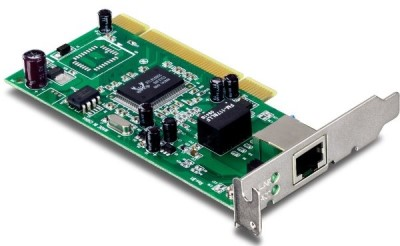
\includegraphics{img/interfaceReseau.jpg}
\caption{interfaceReseau.jpg}
\end{figure}

    \begin{enumerate}
\def\labelenumi{\arabic{enumi}.}
\setcounter{enumi}{1}
\tightlist
\item
  Liaison par onde avec une interface wifi.
\end{enumerate}

    \begin{figure}
\centering
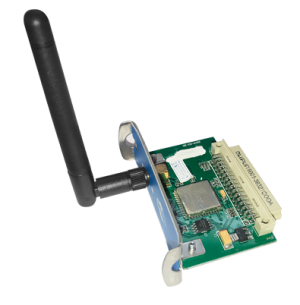
\includegraphics{img/interfaceWifi.png}
\caption{interfaceWifi.png}
\end{figure}

    \hypertarget{remarque}{%
\subsection{Remarque}\label{remarque}}

Il existe également des interfaces réseaux logicielles que l'on
rencontre dans les logiciels de virtualisation. L'interface réseau
virtuelle est reliée à l'interface réseau physique qui peut alors
recevoir et envoyer des données.

\hypertarget{adresse-matuxe9rielle-mac}{%
\subsection{Adresse matérielle
(MAC)}\label{adresse-matuxe9rielle-mac}}

Une \textbf{interface réseau} possède une adresse matérielle ou adresse
MAC (Material Access Control) qui est unique.

Elle se code sur 6 octets notés en hexadécimal : dc:a6:32:42:1a:23 est
l'adresse MAC de la carte réseau d'un raspberry Pi.

    \hypertarget{ruxe9seau-local-lan}{%
\section{Réseau local (LAN)}\label{ruxe9seau-local-lan}}

Un réseau local est un ensemble d'appareils qui sont reliés entre aux et
pouvant s'envoyer et recevoir des données. Au delà de 2 machines, la
connexion ne peut pas se faire directement entre les appareils et
nécessite un \textbf{switch} qui permet de connecter plusieurs
appareils.

    \begin{figure}
\centering
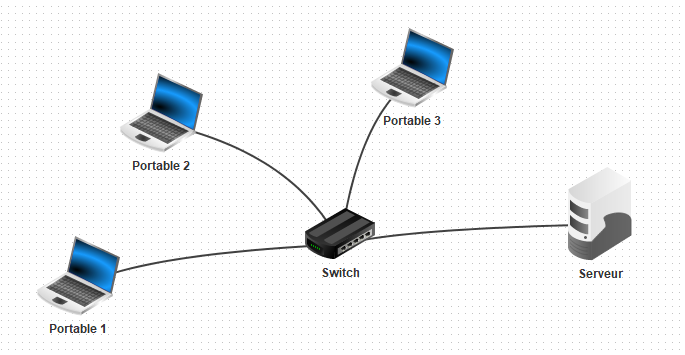
\includegraphics{img/lan_1.png}
\caption{lan\_1.png}
\end{figure}

    \hypertarget{remarque}{%
\subsection{Remarque}\label{remarque}}

Chez les particuliers, c'est la box internet qui remplit le rôle de
switch. Elle permet également aux smartphone de rejoindre le réseau
local via le wifi.

\hypertarget{protocole}{%
\section{Protocole}\label{protocole}}

Un protocole est un ensemble de règles qui permettent
d'\textbf{établir}, \textbf{mener et terminer} une communication entre
deux appareils.

Pour communiquer, les machines doivent suivent des règles qui leurs
permettent :

\begin{itemize}
\tightlist
\item
  de communiquer, c'est à dire qu'elles peuvent s'envoyer et recevoir
  des données;
\item
  d'être identifiées pour que les données soient envoyées sans erreur
  aux bonnes machines;
\item
  de s'assurer que toutes les données sont bien arrivées et dans
  l'ordre;
\item
  d'utiliser des applications utilisant le réseau comme un navigateur
  web.
\end{itemize}

Lorsque les machines sont reliées à un réseau local, le
\textbf{protocole réseau (ethrnet, arp)} utilisant les adresses
matérielles MAC permet aux machines d'être identifiées sur le réseau
local.

    \hypertarget{internet}{%
\section{Internet}\label{internet}}

Le mot \textbf{Internet} est un mot valise issu de l'anglais
(\textbf{inter}connected \textbf{net}work) et qui signifie
\textbf{Interconnexion de réseaux}.

Si 2 machines n'appartiennent pas à un même réseau mais souhaitent
communiquer entre elles, il faut un modèle qui relie les deux réseaux
distants. C'est le \textbf{modèle internet}.

Le \textbf{modèle internet} utilise le \textbf{protocole IP}. Pour ce
faire, les différentes machines ont une \textbf{adresse logique} IPv4 ou
IPv6 qui leur permet d'être identifiées sur leur réseau.

Le protocole IP peut assurer la communication entre deux réseaux
distants avec des \textbf{routeurs}.

    \begin{figure}
\centering
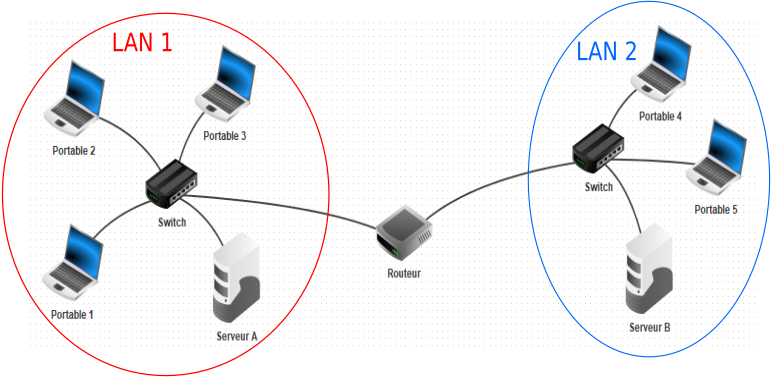
\includegraphics{img/lan_1_et_2.png}
\caption{lan\_1\_et\_2.png}
\end{figure}

    Associé au protocole IP, le \textbf{protocole TCP} assure le transport
de messages de longueur arbitraire en s'assurant qu'ils arrivent
correctement et dans l'ordre jusqu'au destinataire.

Le modèle internet se décompose en 4 couches: - La couche
\textbf{liaison} qui utilise le protocole \textbf{ethernet} - La couche
\textbf{internet} qui utilise le protocole \textbf{IP} - La couche
\textbf{transport} qui utilise le protocole \textbf{TCP} - La couche
\textbf{application} qui utilise les protocoles des programmes utilisés.

    \hypertarget{la-couche-liaison-protocole-ethernet}{%
\section{La couche liaison : protocole
ethernet}\label{la-couche-liaison-protocole-ethernet}}

La couche \textbf{liaison} est la couche la plus basse du modèle
internet. Les interfaces réseaux (carte, wifi) possèdent chacune une
adresse matérielle unique. Elles utilisent le protocole
\textbf{ethernet} pour communiquer d'une interface à l'autre.

Lorsqu'une machine souhaite communiquer avec une autre machine, elle
envoie via son interface réseau, un paquet d'octets appelé \textbf{trame
ethernet}. Cette \textbf{trame} contient l'adresse MAC de destination,
l'adresse MAC de la source et quelques données.

    \begin{figure}
\centering
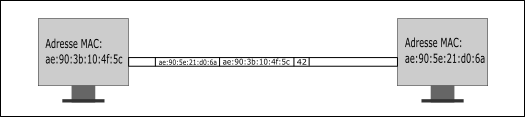
\includegraphics{img/ethernet.png}
\caption{ethernet.png}
\end{figure}

    L'interface réseau d'adresse MAC ae:90:3b:10:4f:5c envoie une trame à
l'interface réseau d'adresse MAC ae:90:5e:21:d0:6a

    \hypertarget{la-couche-internet-protocole-ip}{%
\section{La couche internet : protocole
IP}\label{la-couche-internet-protocole-ip}}

La couche \textbf{internet} se charge de relier les réseaux entre eux
via des dispositifs spécialisés comme les routeurs.

Le \textbf{protocole IP} implique que chaque machine d'un même réseau
réseau ait un identifiant unique appelé adresse IP.

Il existe deux types d'adresses IP:

\begin{itemize}
\tightlist
\item
  l'adresse IPv4 codée sur 4 octets soit 32 bits noté en décimal séparés
  par des \textbf{.}
\item
  l'adresse IPv6 codée sur 16 octets soit 128 bits noté en hexadécimal
  séparés par \textbf{:}
\end{itemize}

Un \textbf{réseau} est caractérisé par 2 adresses IP : l'\textbf{adresse
réseau} et le \textbf{masque de réseau}. Le masque de réseau détermine
le nombre de machines qui pourront se connecter au réseau et ainsi
définit la plage d'adresses à utiliser dans le réseau.

Le masque de réseau est une adresse de 32 bits constituée d'une suite de
bits tous égaux à 1 suivis de bits tous égaux à 0. Il se note soit sur 4
octets soit au format CIDR c'est à dire un nombre qui donne la quatitié
de bits égaux à 1.

\hypertarget{exemple}{%
\subsection{Exemple}\label{exemple}}

Soit un réseau d'adresse \(192.168.0.0\) de masque de sous-réseau
\(255.255.255.0\).

En binaire, le masque de sous-réseau est : \(1111\) \(1111\) \(1111\)
\(1111\) \(1111\) \(1111\) \(0000\) \(0000\) ce qui signifie qu'il y a
24 bits égaux à 1.

On peut donc noter l'adresse réseau et son masque par \(192.168.0.0/24\)

Ce masque permet d'avoir sur le réseau \(2^{8}=256\) adresses IP
distinctes.

    \hypertarget{adresse-ruxe9seau}{%
\subsection{Adresse réseau}\label{adresse-ruxe9seau}}

Lorsqu'on connaît l'adresse IP d'ne machine dans un réseau local et le
masque de réseau, il possible en appliquant un ET binaire, bit par bit,
d'obtenir l'adresse du réseau.

\hypertarget{exemple}{%
\subsection{Exemple}\label{exemple}}

Une machine a pour adresse IP 192.168.15.24/23

L'adresse \(192.168.15.24\) se note
\(1100 0000.1010 1000.0000 1111.0001 1000\) en binaire et le masque se
note \(1111 1111.1111 1111.1111 1110.0000 0000\).

L'application d'un ET binaire entre ces 2 adresses nous donne l'adresse
du réseau:

    \begin{figure}
\centering
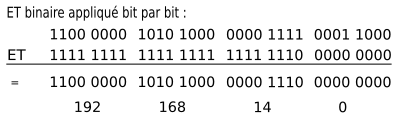
\includegraphics{img/et-binaire.png}
\caption{et-binaire.png}
\end{figure}

    L'adresse du réseau est donc \(192.168.14.0\) et contient \(2^{9}=512\)
adresses IP.

    Une machine dans un réseau local connait les adresses IP de plusieurs
services réseau:

\begin{itemize}
\tightlist
\item
  L'adresse IP de broadcast qui permet d'envoyer un message à toutes les
  machines du réseau en même temps;
\item
  L'adresse IP de la passerelle ou routeur pour accéder à d'autres
  réseaux (internet);
\item
  L'adresse du serveur DHCP qui attribue automatiquement les adresses IP
  aux machines du réseau;
\item
  L'adresse IP du serveur DNS qui effectue la résolution des noms de
  domaine, c'est à dire transforme un nom de domaine en adresse IP;
\item
  L'adresse IP d'un serveur de domaine qui authentifie les utilisateurs
  à se connecter aux machines du réseau.
\end{itemize}

\hypertarget{remarques}{%
\subsection{Remarques}\label{remarques}}

\begin{enumerate}
\def\labelenumi{\arabic{enumi}.}
\item
  Le nombre d'adresse en IPv4 est devenu insuffisant pour fournir le
  monde entier en adresses. Le passage en IPv6 permet d'attribuer
  beaucoup plus d'adresses. Quoi qu'il en soit, cela ne change pas le
  protocole IP basé sur des adresses logiques.
\item
  Il existe un service, \textbf{DHCP}, qui attribue les adresses IP aux
  machines d'un même réseau. Ce service s'assure qu'aucune machine n'ait
  la même adresse IP. Le service DHCP est installé sur un serveur.
\end{enumerate}

Le second rôle du \textbf{protocole IP} est le routage des données à
travers différents réseaux.

    \begin{figure}
\centering
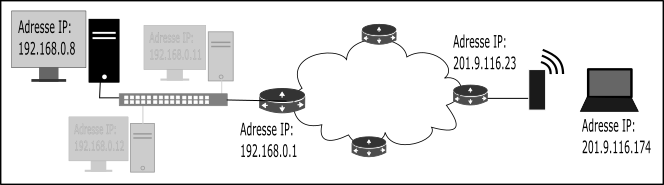
\includegraphics{img/reseauIP.png}
\caption{reseauIP.png}
\end{figure}

    Les routeurs reliant les réseaux sont aussi appelés des
\textbf{passerelles}.

Pour mener à bien ce routage, les données à transmettre sont encapsulées
dans un paquet IP qui contient l'adresse IP source, l' adresse IP du
destinataire et les données à transmettre.

    \hypertarget{la-couche-transport---protocole-tcp}{%
\section{La couche transport - protocole
TCP}\label{la-couche-transport---protocole-tcp}}

La couche \textbf{transport}, via le protocole TCP, s'assure du bon
acheminement des données pour être utilisés par les programmes.

\begin{itemize}
\tightlist
\item
  Le protocole TCP s'assure que les paquets IP arrivent au bon
  programme;
\item
  Le protocole TCP s'assure que les paquets IP sont tous arrivés.
\end{itemize}

\hypertarget{arrivuxe9-uxe0-bon-port}{%
\subsection{Arrivé à bon port}\label{arrivuxe9-uxe0-bon-port}}

En pratique, une machine dans un réseau exécute des programmes et
sollicite un service réseau. Si le protocole IP assure la communication
avec les adresses IP, comment les données arrivent-elles aux bons
programmes ?

C'est le rôle de la couche transport et du protocole TCP. Celui-ci
ajoute aux paquets IP deux nombres : les \textbf{numéros de port}.

\begin{itemize}
\tightlist
\item
  un \textbf{port source} pour identifier le programme qui demande le
  service;
\item
  un \textbf{port destinataire} pour identifier le programme sur le
  serveur qui reçoit la demande.
\end{itemize}

Les paquets IP sont donc encapsulés et deviennent des
\textbf{datagrammes} qui contiennent le port source, le port
destinataire et le paquet IP.

La connexion d'un client à un serveur avec le protocole TCP se réalise
en 3 temps avant d'envoyer les données.

\begin{enumerate}
\def\labelenumi{\arabic{enumi}.}
\tightlist
\item
  le client choisit un \textbf{numéro de séquence} aléatoire (1234 par
  exemple) et envoie au serveur un paquet étiqueté \textbf{SYN}
  indiquant le numéro choisi.
\item
  le serveur reçoit le paquet,\textbf{incrémente le numéro de séquence}
  (1235) et choisit aussi un numéro aléatoire (190) et envoie le tout
  dans un paquet étiqueté \textbf{SYN-ACK}.
\item
  le client reçoit alors le paquet SYN-ACK, incrémente les 2 numéros
  (1236 et 191) et envoie le tout dans un paquet \textbf{ACK}. La
  connexion est établie.
\end{enumerate}

    \begin{figure}
\centering
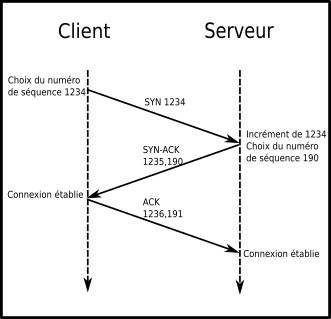
\includegraphics{img/TCP-SYN-ACK.png}
\caption{TCP-SYN-ACK.png}
\end{figure}

    La couche transport n'envoie pas les données en une fois ! Les données
sont découpées, envoyées puis réassemblées par la machine de
destination. Le protocole TCP va incrémenter les numéros de séquence
jusqu'à la fin de la transmission permettant d'éviter les erreurs et le
renvoi de données éventuellement perdues.

\hypertarget{remarque}{%
\subsection{Remarque}\label{remarque}}

Les ports compris entre 0 et 1024 sont réservés pour des services
réseaux. - Le web utilise les ports 80 et 443. Dès que l'on navigue sur
le web, les ports de destinations sont 80 ou 443 associés à un port
source supérieur à 1024. - La résolution d'adresse sur le web fait appel
à un serveur DNS qui se charge de transformer une url en adresse IP. Le
port destination utilisé est le 53. - Au démarrage de la machine,
celle-ci reçoit une adresse IP grace au serveur DHCP. Cette attribution
se fait sur le port 67.

    \hypertarget{la-couche-application}{%
\section{La couche application}\label{la-couche-application}}

C'est la couche la plus haute et elle concerne les différents programmes
qui ont besoin de données situées sur le réseau ou internet.

\hypertarget{exemple}{%
\subsection{Exemple}\label{exemple}}

On souhaite afficher la page web : https://fr.wikipedia.org/

\begin{itemize}
\tightlist
\item
  Une requête au serveur DNS est envoyée. C'est la couche Application.
\item
  Le protocole TCP de la couche transport crée un datagramme en ajoutant
  les ports dont le 53 comme port de destination;
\item
  Le protocole IP de la couche internet crée un paquet IP en ajoutant au
  datagramme les adresses IP de la machine source et du serveur DNS.
\item
  Le protocole ethernet de la couche liaison crée une trame en ajoutant
  les adresses matérielles (MAC) des interfaces réseaux.
\end{itemize}

    \begin{figure}
\centering
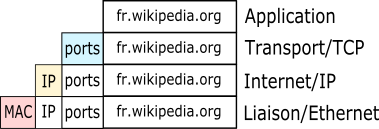
\includegraphics{img/couches.png}
\caption{couches.png}
\end{figure}


    % Add a bibliography block to the postdoc
    
    
    
\end{document}
